\documentclass{article}
\usepackage[T1]{fontenc}
\usepackage{lmodern}
\usepackage{graphicx}
\usepackage{amsmath,amssymb}
\usepackage[a4paper,margin=2cm]{geometry}
\usepackage[absolute,overlay]{textpos}
\setlength{\TPHorizModule}{1mm}
\setlength{\TPVertModule}{1mm}
\usepackage[indonesian]{babel}
\usepackage{hyperref}
\setlength{\emergencystretch}{2em}
% unit: Halaman 28

\begin{document}

% === Halaman 28 (llm) ===

\begin{itemize}
    \item \textit{Keystream generator} menerima masukan sebuah umpan (\textit{seed}) $U$. Luaran dari prosedur merupakan fungsi dari $U$ (lihat Gambar 2). Pengirim dan penerima harus memiliki umpan $U$ yang sama. Umpan $U$ ini harus dijaga kerahasiaannya. Umpan $U$ dapat dianggap sebagai kunci eksternal.
    \item \textit{Keystream generator} menghasilkan bit-bit kunci yang di-XOR-kan dengan bit plainteks.
\end{itemize}

\vspace{40mm}

\textbf{Gambar 2} \textit{Cipher} aliran dengan pembangkit bit kunci-alir yang bergantung pada kunci $U$ [MEY82].

% deskripsi: Diagram blok sistem kriptografi stream cipher yang menunjukkan proses enkripsi oleh pengirim dan dekripsi oleh penerima menggunakan Keystream Generator dengan seed U.
% bbox normalisasi: [0.1800, 0.4100, 0.8600, 0.8500]
\begin{textblock*}{142.80mm}(37.80mm,121.77mm)
\noindent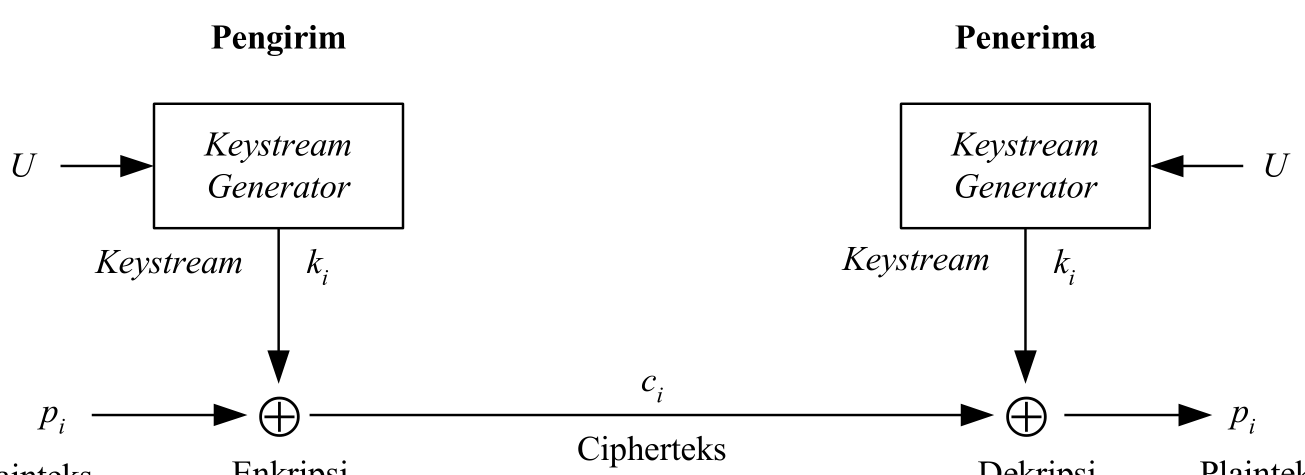
\includegraphics[width=142.80mm,height=130.68mm]{../../images/llm/page_028_img_01.png}%
\end{textblock*}

\end{document}
